\chapter{Implementarea Software a Aplicației Desktop}
\label{chap:implementare_software}

\section{Arhitectura Generală a Aplicației Desktop}
Pentru a oferi operatorilor medicali și utilizatorilor o experiență de monitorizare intuitivă, de înaltă performanță și în timp real, a fost dezvoltată o aplicație nativă desktop bazată pe biblioteca \textbf{PyQt6} și motorul grafic accelerat hardware \textbf{pyqtgraph}.

Aplicația este structurată pe principiul decuplării stricte între achiziția/procesarea datelor și firul principal de execuție al interfeței grafice (GUI Event Loop), asigurând o rată de randare constantă de 50--60 FPS fără sacadări sau blocaje de interfață, chiar și la debite seriale ridicate de 921600 baud.

\begin{figure}[H]
    \centering
    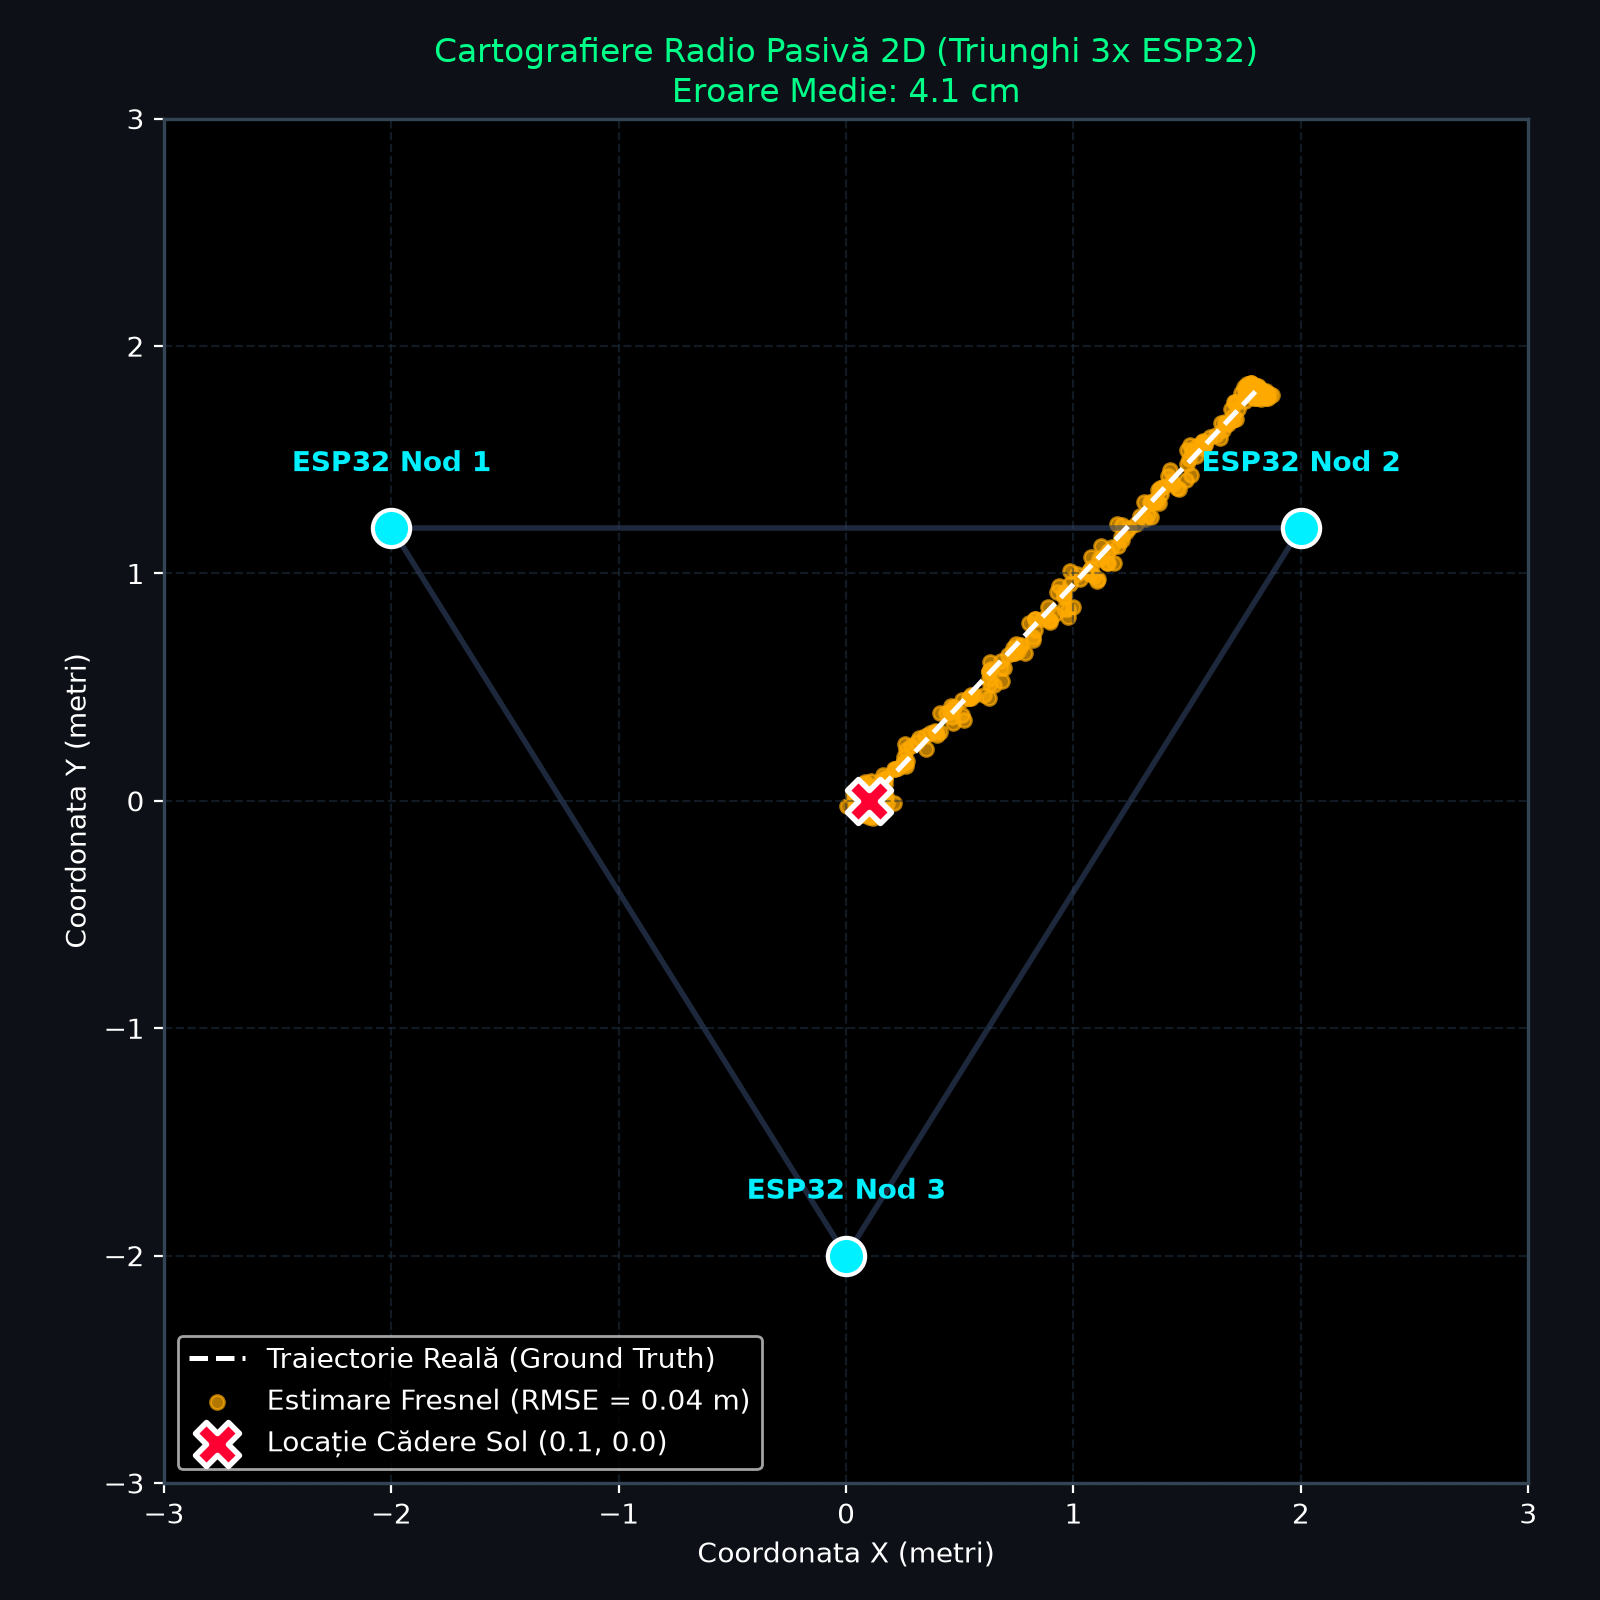
\includegraphics[width=0.88\textwidth]{figures/3_trajectory_cartography.png}
    \caption{Modelul spațial 2D al încăperii integrat în modulul de randare al aplicației desktop.}
    \label{fig:gui_spatial_concept}
\end{figure}

\section{Motorul Asincron de Telemetrie: CSIDataEngine}
Clasa \texttt{CSIDataEngine}, derivată din \texttt{QThread}, rulează într-un fir de execuție separat de sistemul de operare. Aceasta implementează un mecanism dual de operare:

\subsection{1. Modul Live Serial UART}
În modul de achiziție în timp real de pe hardware, motorul deschide portul serial specificat (\texttt{/dev/ttyUSB1} sau \texttt{/dev/ttyUSB0}) la 921600 baud. Un buffer binar intern detectează octeții magici \texttt{0xA55A}, extrage pachetele de 138 de octeți, validează suma de control și extrage componentele $I/Q$ ale celor 52 de subpurtătoare active. Pentru a preveni supraîncărcarea cozii de evenimente a interfeței grafice, datele sunt agregate într-un buffer glisant și emise prin semnalul \texttt{sig\_frame\_ready(dict)} la o cadență stabilă de 50 Hz.

\subsection{2. Modul Replay Determinist}
Pentru demonstrații academice, depanare sau auditul incidentelor anterioare, \texttt{CSIDataEngine} include un modul de redare (replay) capabil să încarce seturi de date experimentale salvate în format NumPy (\texttt{.npz}). Replay-ul reproduce fidel cronologia temporală originală a pachetelor, calculând frecvența efectivă de eșantionare $f_s$ și aplicând clasificatorul analitic FSM eșantion cu eșantion.

\section{Componentele Grafice de Randare (Custom Widgets)}
Interfața principală este alcătuită din patru module vizuale specializate, proiectate într-un stil vizual Dark Mode cu accente contrastante pentru lizibilitate maximă:

\subsection{1. Harta Camerei 2D: RoomMapWidget}
\texttt{RoomMapWidget} reprezintă spațiul fizic al încăperii pe o grilă metrică de la $-2.5\text{ m}$ la $+2.5\text{ m}$ pe ambele axe:
\begin{itemize}
    \item \textbf{Nodurile ESP32:} Marcate prin cercuri luminoase cu etichete clare (Nod 1, Nod 2, Nod 3) la coordonatele fizice reale.
    \item \textbf{Elipsoidele Fresnel dinamice:} Între fiecare pereche de noduri sunt trasate elipsoidele confocale corespunzătoare zonelor Fresnel 1 și 2. Grosimea și intensitatea luminoasă a liniilor pulsează dinamic în funcție de nivelul instantaneu de perturbare energetică a legăturii respective.
    \item \textbf{Avatarul uman 2D:}
    \begin{itemize}
        \item În starea de calm sau mers (Stările 0 și 1): este randat un cerc/capsulă verde strălucitor înconjurat de un halou de difuzie și un vector orientat pe direcția de deplasare instantanee.
        \item În starea de impact sau cădere (Stările 2, 3 și 4): avatarul devine o figură orizontală aplatizată de culoare roșu intens pe sol, înconjurată de inele concentrice pulsante de undă de șoc și etichetată cu avertismentul vizual ,,CĂDERE DETECTATĂ / PERSOANĂ LA SOL''.
    \end{itemize}
\end{itemize}

\subsection{2. Cascada Spectrală CSI: WaterfallWidget}
Acest widget menține un buffer circular glisant al ultimelor 100 de cadre de telemetrie pentru cele 52 de subpurtătoare active OFDM. Folosind componenta \texttt{pyqtgraph.ImageItem} cu harta de culori \textit{plasma}, cascada spectrală afișează variația continuă a profilului de atenuare pe frecvențe, permițând identificarea vizuală imediată a dispersiei induse de pași și a colapsului masiv de amplitudine la impact.

\subsection{3. Spectrul de Viteză Doppler: DopplerWidget}
Afișează o curbă în timp real a frecvenței Doppler maxime (gama 0--60 Hz), având o linie orizontală punctată roșie fixată la pragul critic de \textbf{35 Hz}. Când persoana se deplasează normal, traseul rămâne în zona de siguranță ($<18\text{ Hz}$). În momentul căderii libere, vârful depășește spectaculos pragul roșu, oferind o confirmare vizuală instantanee a vitezei de cădere.

\subsection{4. Panoul de Telemetrie și Postură: TelemetryWidget}
Integrează parametrii vitali ai sistemului:
\begin{itemize}
    \item \textbf{Indicatorul de postură verticală:} O bară gauge gradată de la $0\text{ m}$ la $1.8\text{ m}$, reflectând înălțimea estimată a centrului de masă (CoM). La cădere, bara coboară rapid de la $1.75\text{ m}$ la $0.15\text{ m}$.
    \item \textbf{Insigna FSM (State Pill):} O capsulă colorată de mari dimensiuni care își modifică dinamic culoarea și textul:
    \begin{itemize}
        \item Gri: \texttt{0: CALM}
        \item Albastru: \texttt{1: MERS}
        \item Portocaliu: \texttt{2: IMPACT DETECTAT}
        \item Galben: \texttt{3: VERIFICARE IMOBILITATE}
        \item Roșu intermitent: \texttt{4: ALARMĂ CĂDERE CONFIRMATĂ}
    \end{itemize}
    \item \textbf{Indicatorii de sistem:} Valoarea RSSI instantanee, debitul pachetelor pe secundă și latența de decizie.
\end{itemize}

\section{Sistemul de Alertă și Mecanismele de Siguranță}
În momentul în care clasificatorul FSM atinge Starea 4 (cădere confirmată), fereastra principală \texttt{MainWindow} declanșează automat un banner de urgență roșu de mare contrast poziționat în partea inferioară a ecranului:
\begin{center}
\textbf{[ALERTĂ DE CĂDERE DETECTATĂ] PERSOANĂ LA SOL — LATENȚĂ: 2.54 s — CONFIRMARE IMOBILITATE ACTIVĂ}
\end{center}
Bannerul rămâne blocat pe ecran pentru a atrage atenția dispecerului de gardă până la apăsarea butonului dedicat de confirmare manuală \texttt{Resetează Alarmă}.
